\section{Classification \& Logistic Regression}
\subsection{Binary Classification}
\begin{itemize}
    \item Decision with 2 possible outcomes
    \item Hail in Lausanne (yes/no)
    \item Master admission (admission / no admission)
    \item Based on different data / entity
\end{itemize}

\subsubsection{Decision using Linear Regression}
\begin{itemize}
    \item Train the model with gradient descent
    \item \textbf{Bad Idea!}
    \item Models the response (y) and post process the response to compute the probability
\end{itemize}

\subsubsection{The sigmoid function}
\begin{center}
    $sigmoid(y) = \frac{1}{1 + e^{-y}}$
\end{center}
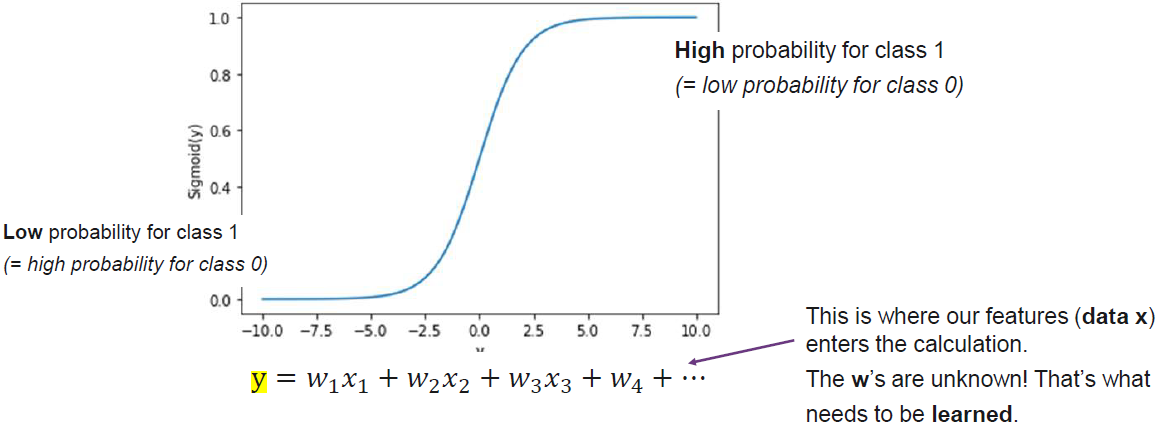
\includegraphics[width=\linewidth]{./img/sigmoid.png}
\textbf{Probabilities}
\begin{itemize}
    \item We can write the estimated probability
    \item For a prediction we can write
\end{itemize}
\begin{center}
    $P(x) = \frac{1}{1 + e^{-(W^{T}x)}}$
\end{center}

\subsubsection{Maximum Likelihood}
\begin{itemize}
    \item Given all the data points (X,Y) we want to maximize the probability that all the predictions are correct.
    \item For each of the training data, we want to maximize the likelihood of correct prediction
    \item We can use Gradient Descent to find W
\end{itemize}